\section{Additional Data} \label{data}
    \subsection{Methyloxirane}
    \begin{figure}
        \centering
        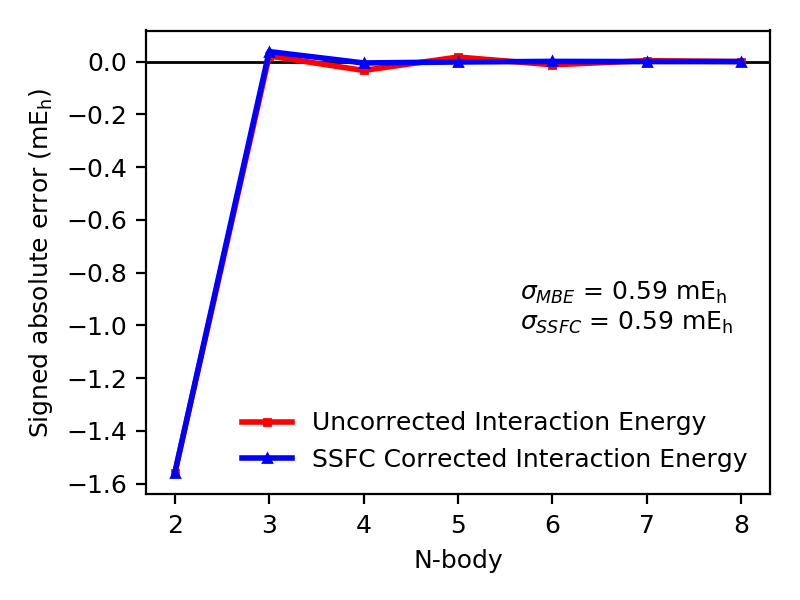
\includegraphics[scale=0.75]{p1/graphs/si/metox_7_b3_int.png}
        \caption{MBE and SSFC of interaction energy for (\textit{S})-methyloxirane in a seven-water solvent shell. Computed with B3LYP/aDZ.}
        \label{metox_7_b3_int}
    \end{figure}
    \begin{figure}
        \centering
        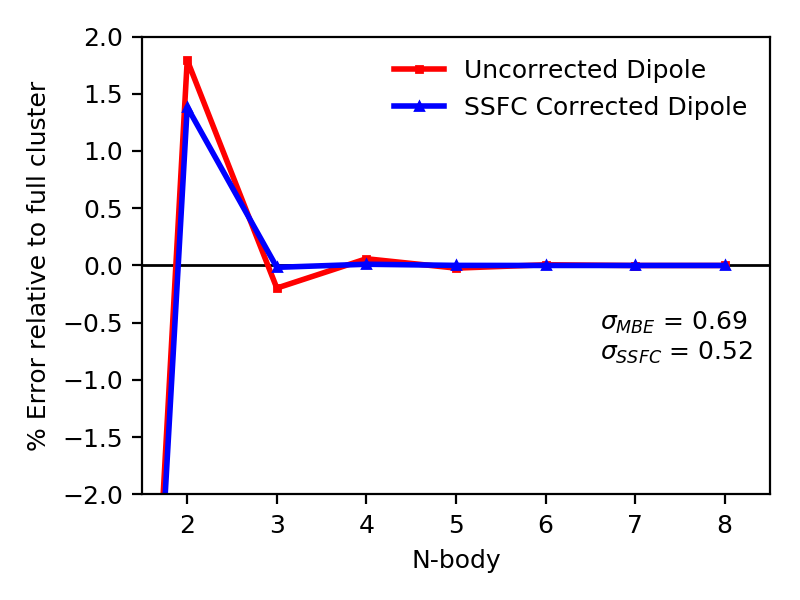
\includegraphics[scale=0.75]{p1/graphs/si/metox_7_b3_dip.png}
        \caption{MBE and SSFC of dipole moment for (\textit{S})-methyloxirane in a seven-water solvent shell. Computed with B3LYP/aDZ.}
        \label{metox_7_b3_dip}
    \end{figure}

    \begin{figure}
        \centering
        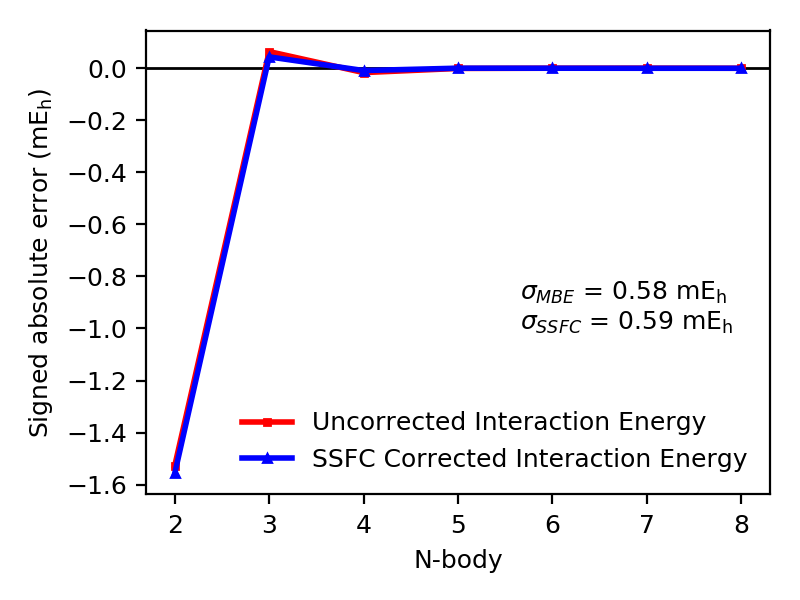
\includegraphics[scale=0.75]{p1/graphs/si/metox_7_tz_int.png}
        \caption{MBE and SSFC of interaction energy for (\textit{S})-methyloxirane in a seven-water solvent shell. Computed with B3LYP/aTZ.}
        \label{metox_7_tz_int}
    \end{figure}
    \begin{figure}
        \centering
        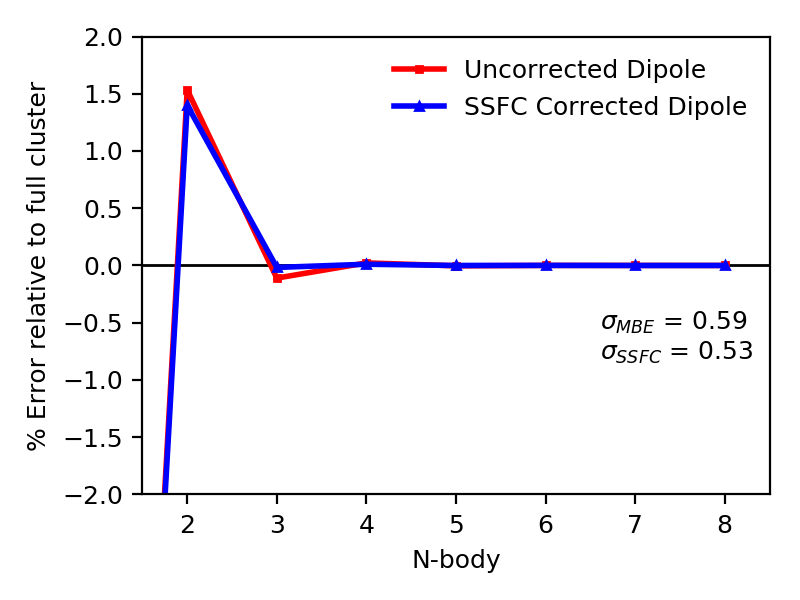
\includegraphics[scale=0.75]{p1/graphs/si/metox_7_tz_dip.png}
        \caption{MBE and SSFC of dipole moment for (\textit{S})-methyloxirane in a seven-water solvent shell. Computed with B3LYP/aTZ.}
        \label{metox_7_tz_dip}
    \end{figure}

    \begin{figure}
        \centering
        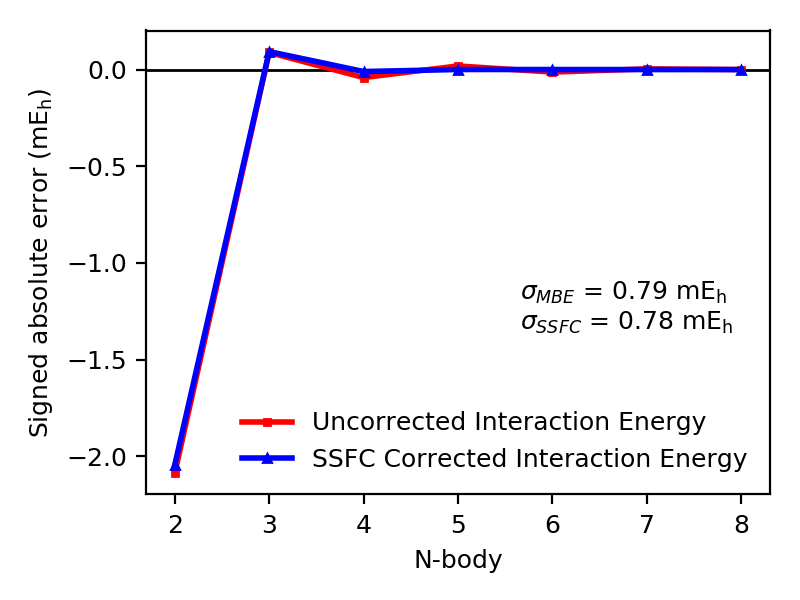
\includegraphics[scale=0.75]{p1/graphs/si/metox_7_cam_int.png}
        \caption{MBE and SSFC of interaction energy for (\textit{S})-methyloxirane in a seven-water solvent shell. Computed with CAM-B3LYP/aDZ.}
        \label{metox_7_cam_int}
    \end{figure}
    \begin{figure}
        \centering
        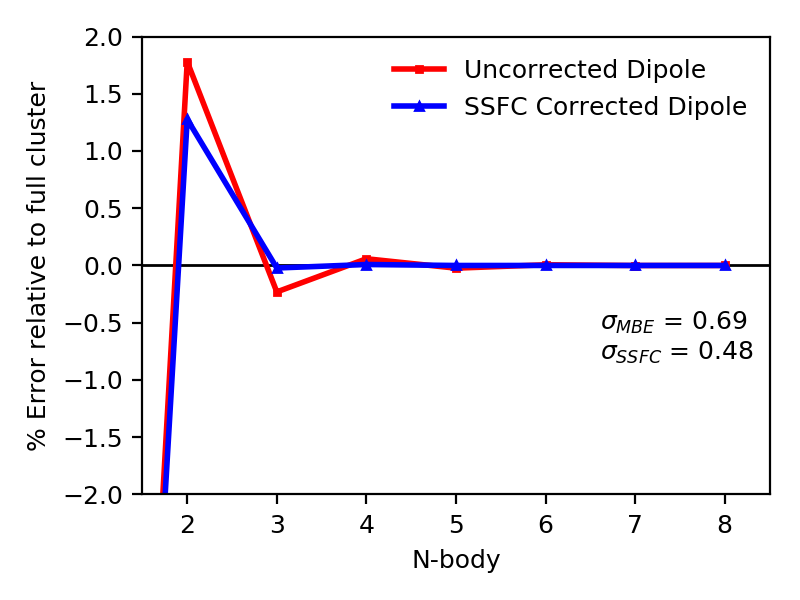
\includegraphics[scale=0.75]{p1/graphs/si/metox_7_cam_dip.png}
        \caption{MBE and SSFC of dipole moment for (\textit{S})-methyloxirane in a seven-water solvent shell. Computed with CAM-B3LYP/aDZ.}
        \label{metox_7_cam_dip}
    \end{figure}
    \begin{figure}
        \centering
        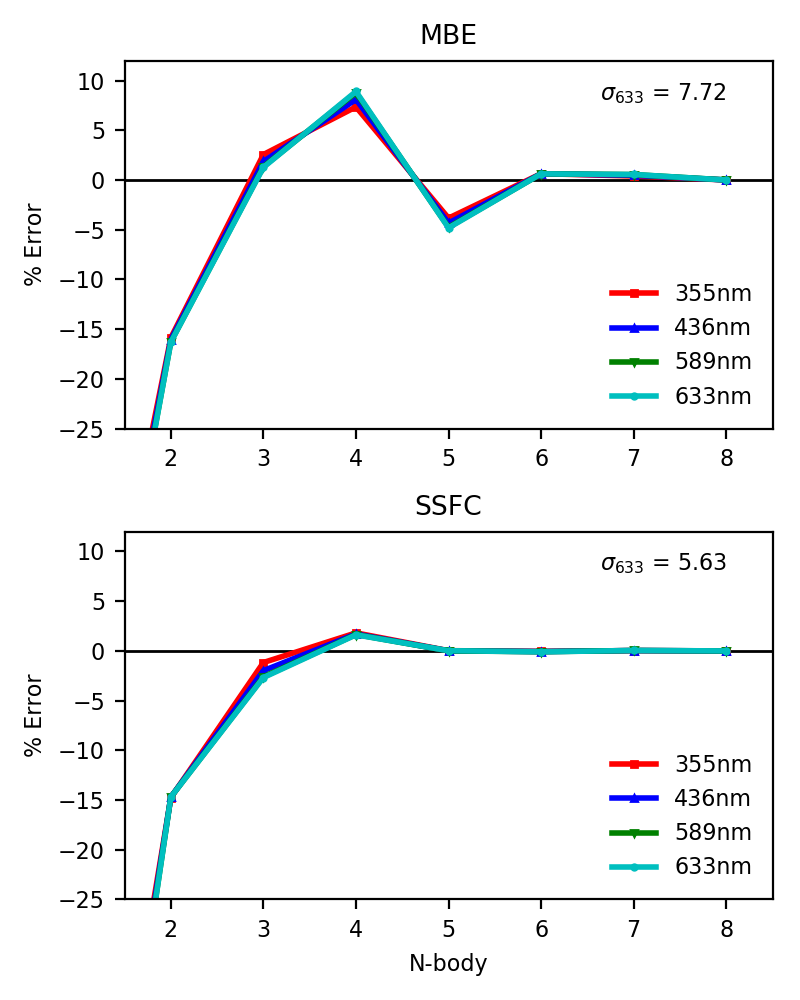
\includegraphics[scale=0.75]{p1/graphs/si/metox_7_cam_rot.png}
        \caption{MBE and SSFC of specific rotation for (\textit{S})-methyloxirane in a seven-water solvent shell. Computed with CAM-B3LYP/aDZ.}
        \label{metox_7_cam_rot}
    \end{figure}

    \begin{figure}
        \centering
        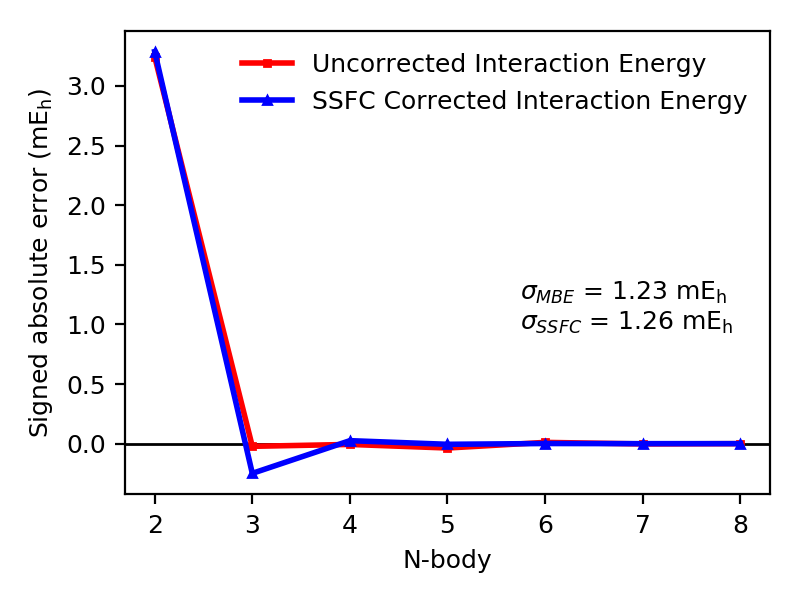
\includegraphics[scale=0.75]{p1/graphs/si/metox2_7_int.png}
        \caption{MBE and SSFC of interaction energy for snapshot \#2 of (\textit{S})-methyloxirane in a seven-water solvent shell. Computed with CAM-B3LYP/aDZ.}
        \label{metox2_7_int}
    \end{figure}
    \begin{figure}
        \centering
        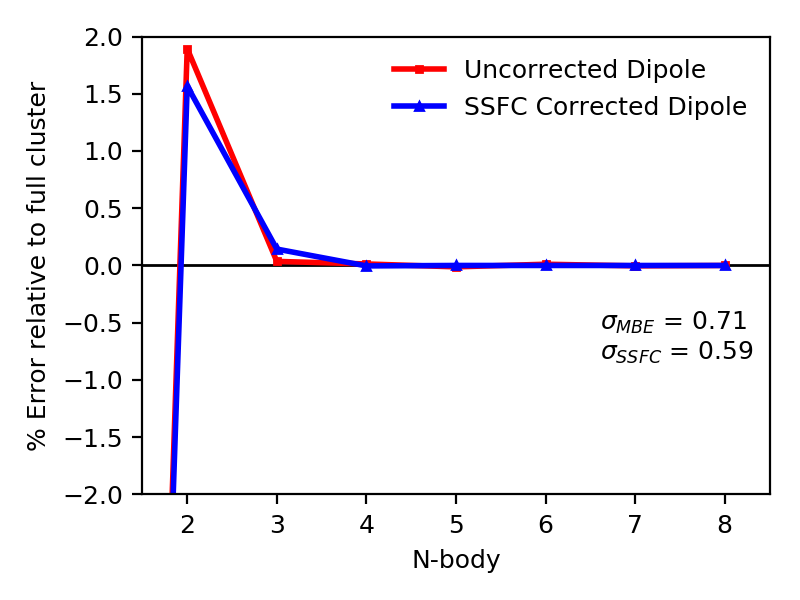
\includegraphics[scale=0.75]{p1/graphs/si/metox2_7_dip.png}
        \caption{MBE and SSFC of dipole moment for snapshot \#2 of (\textit{S})-methyloxirane in a seven-water solvent shell. Computed with CAM-B3LYP/aDZ.}
        \label{metox2_7_dip}
      \end{figure}
    \begin{figure}
            \centering
            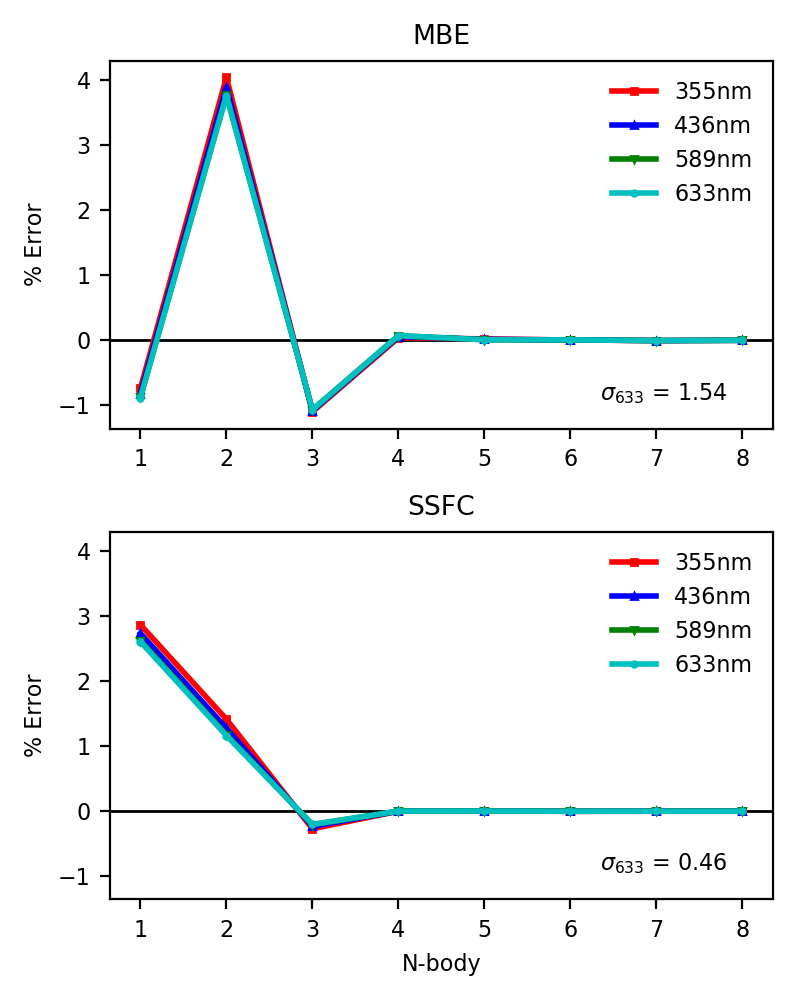
\includegraphics[scale=0.75]{p1/graphs/metox2_7_pol.png}
            \caption{(\textit{S})-methyloxirane}
        \caption{MBE and SSFC of dynamic polarizabilities for
          snapshot \#2 of (\textit{S})-methyloxirane in a seven-water solvent shell. Computed with CAM-B3LYP/aDZ.}
            \label{metox2_pol}
    \end{figure}
    \begin{figure}
        \centering
        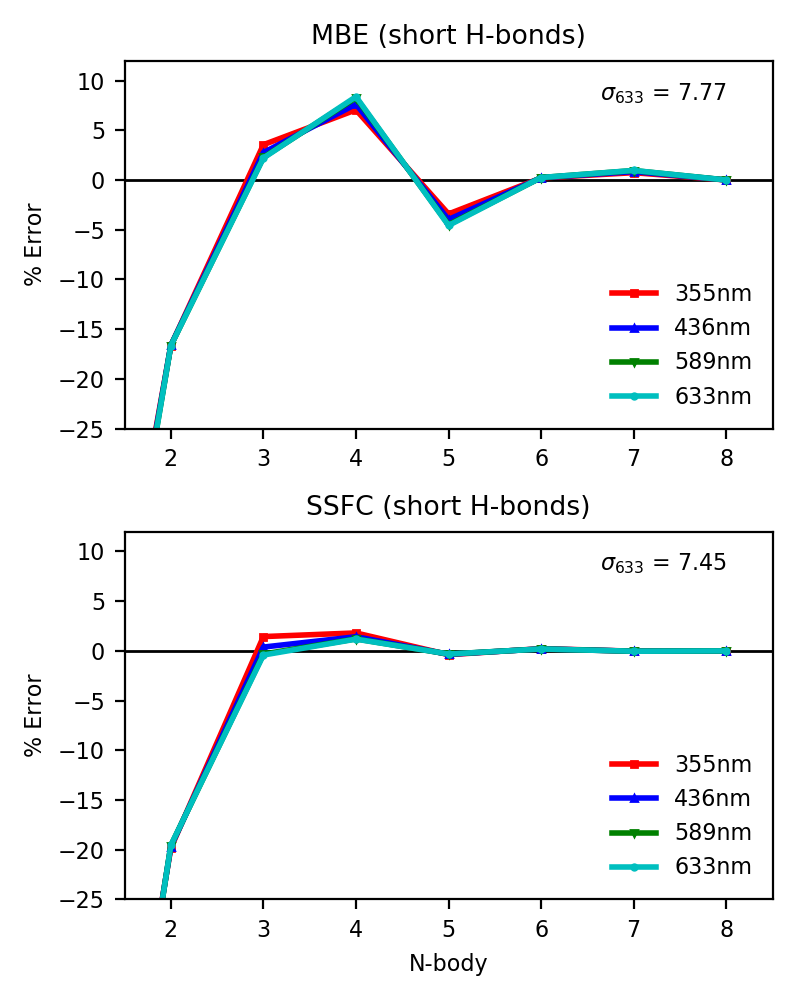
\includegraphics[scale=0.75]{p1/graphs/si/metox_7_short_2_rot.png}
        \caption{MBE and SSFC of specific rotation of (\textit{S})-methyloxirane in a seven-water solvent shell and two manually reduced H-bonds. Computed with CAM-B3LYP/aDZ.}
        \label{metox7_short2_rot.png}
      \end{figure}
    \begin{figure}
        \centering
        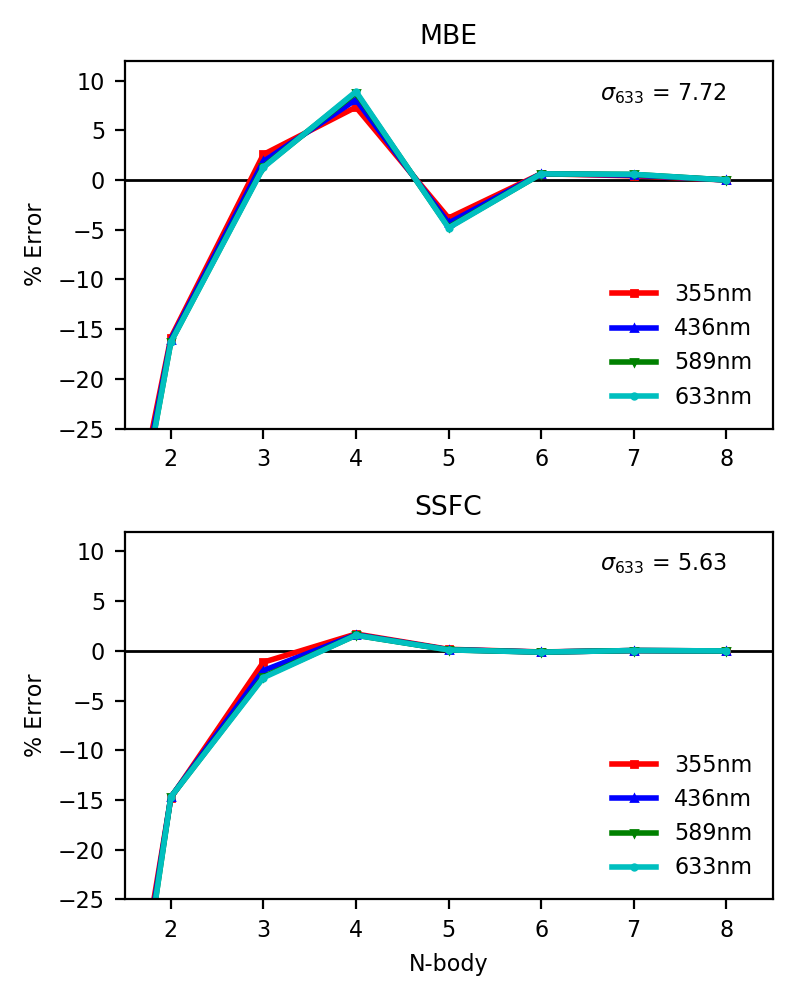
\includegraphics[scale=0.75]{p1/graphs/si/metox_7_tight.png}
        \caption{MBE and SSFC of specific rotation of (\textit{S})-methyloxirane in a seven-water solvent shell using ``tight'' convergence criteria and ``fine'' grids. Computed with CAM-B3LYP/aDZ.}
        \label{metox7_tight.png}
      \end{figure}
    \begin{figure}
        \centering
        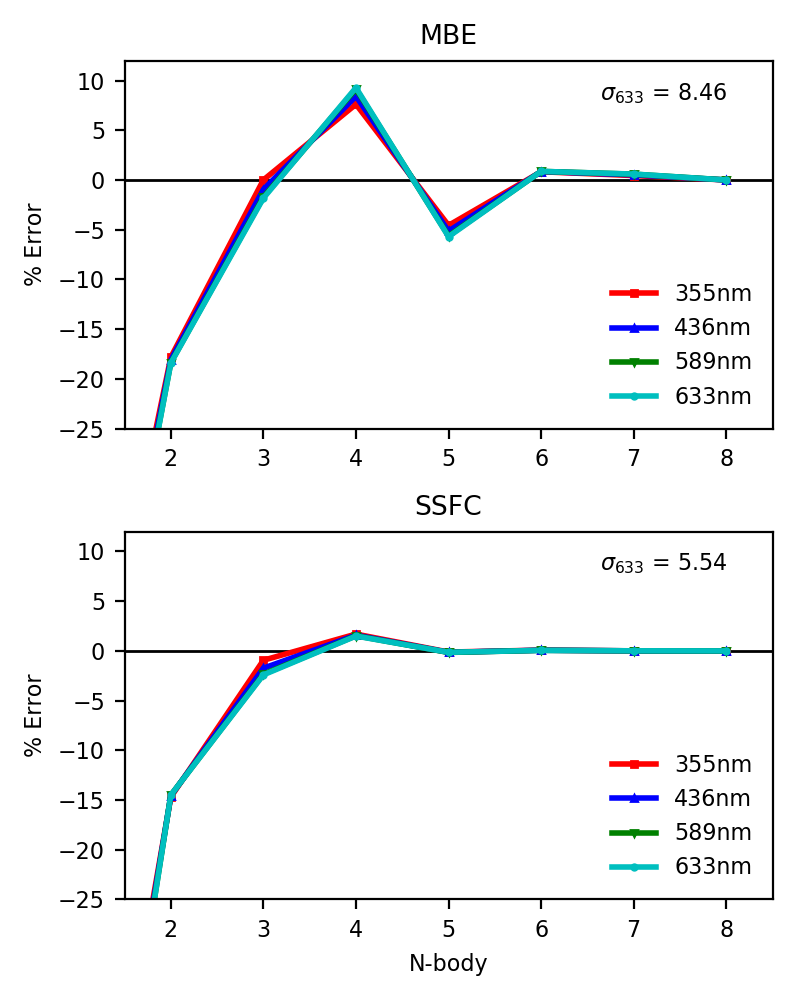
\includegraphics[scale=0.75]{p1/graphs/si/metox_7_noprune.png}
        \caption{MBE and SSFC of specific rotation of (\textit{S})-methyloxirane in a seven-water solvent shell and unpruned ``fine'' grids. Computed with CAM-B3LYP/aDZ.}
        \label{metox7_noprune.png}
      \end{figure}

\clearpage
    \subsection{Methylthiirane}
    \begin{figure}
        \centering
        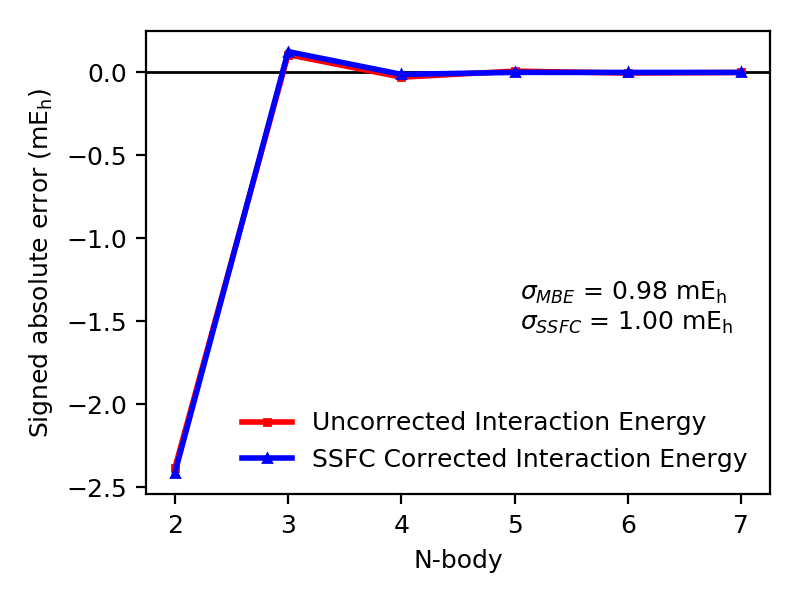
\includegraphics[scale=0.75]{p1/graphs/si/metthi_6_b3_int.png}
        \caption{MBE and SSFC of interaction energy for (\textit{S})-methylthiirane in a six-water solvent shell. Computed with B3LYP/aDZ.}
        \label{metthi_6_b3_int}
    \end{figure}
    \begin{figure}
        \centering
        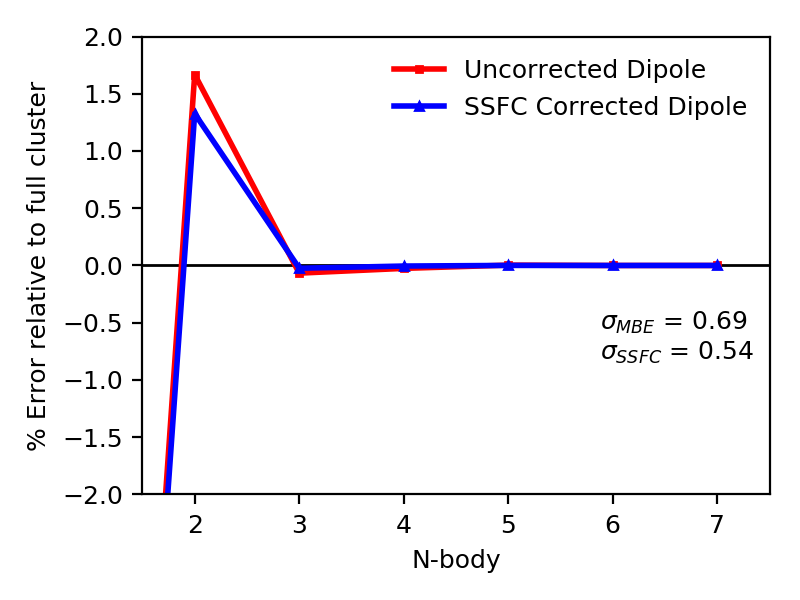
\includegraphics[scale=0.75]{p1/graphs/si/metthi_6_b3_dip.png}
        \caption{MBE and SSFC of dipole moment for (\textit{S})-methylthiirane in a six-water solvent shell. Computed with B3LYP/aDZ.}
        \label{metthi_6_b3_dip}
    \end{figure}

    \begin{figure}
        \centering
        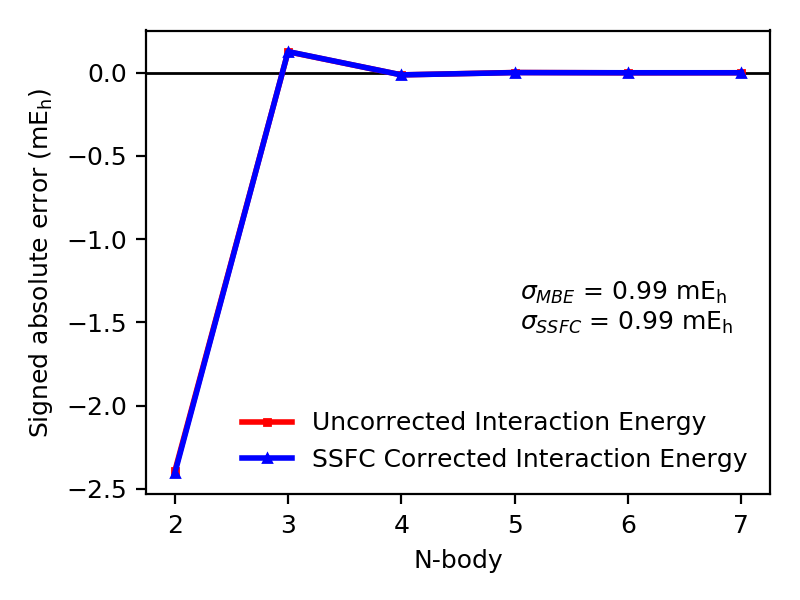
\includegraphics[scale=0.75]{p1/graphs/si/metthi_6_tz_int.png}
        \caption{MBE and SSFC of interaction energy for (\textit{S})-methylthiirane in a six-water solvent shell. Computed with B3LYP/aTZ.}
        \label{metthi_6_tz_int}
    \end{figure}
    \begin{figure}
        \centering
        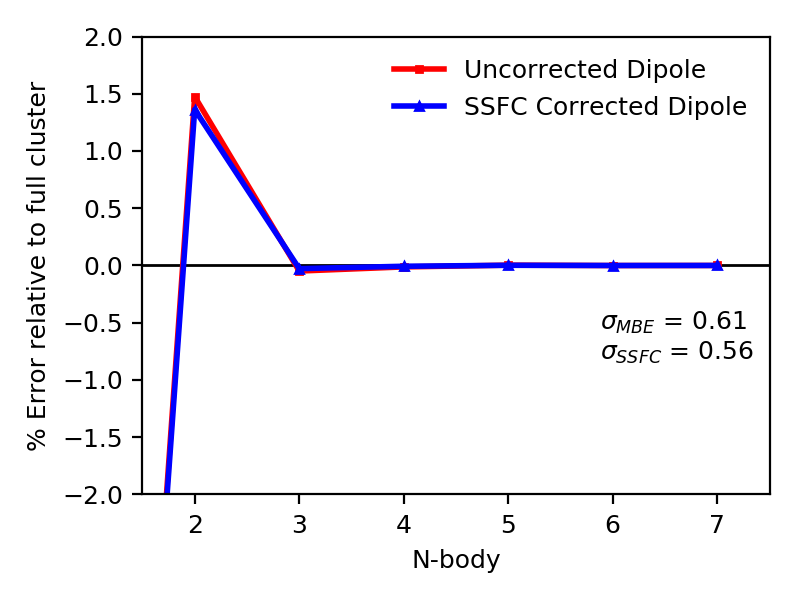
\includegraphics[scale=0.75]{p1/graphs/si/metthi_6_tz_dip.png}
        \caption{MBE and SSFC of dipole moment for (\textit{S})-methylthiirane in a six-water solvent shell. Computed with B3LYP/aTZ.}
        \label{metthi_6_tz_dip}
    \end{figure}

    \begin{figure}
        \centering
        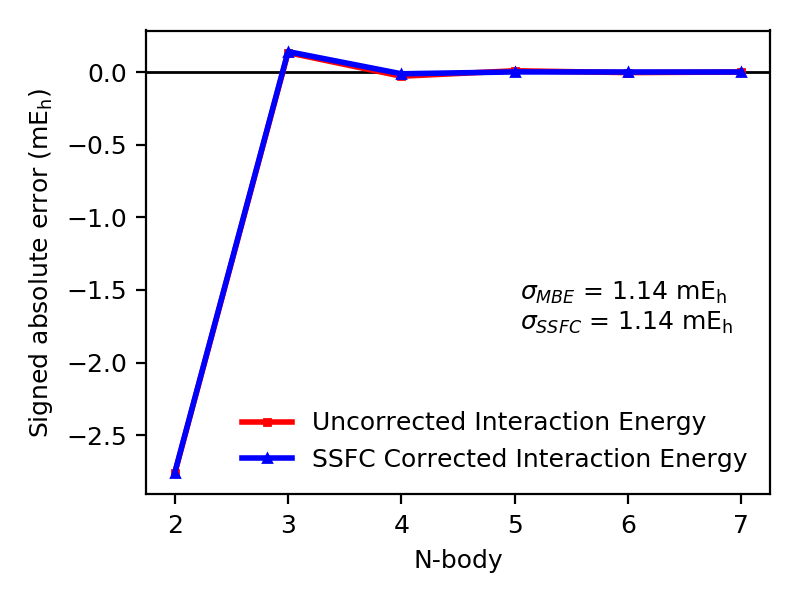
\includegraphics[scale=0.75]{p1/graphs/si/metthi_6_cam_int.png}
        \caption{MBE and SSFC of interaction energy for (\textit{S})-methylthiirane in a six-water solvent shell. Computed with CAM-B3LYP/aDZ.}
        \label{metthi_6_cam_int}
    \end{figure}
    \begin{figure}
        \centering
        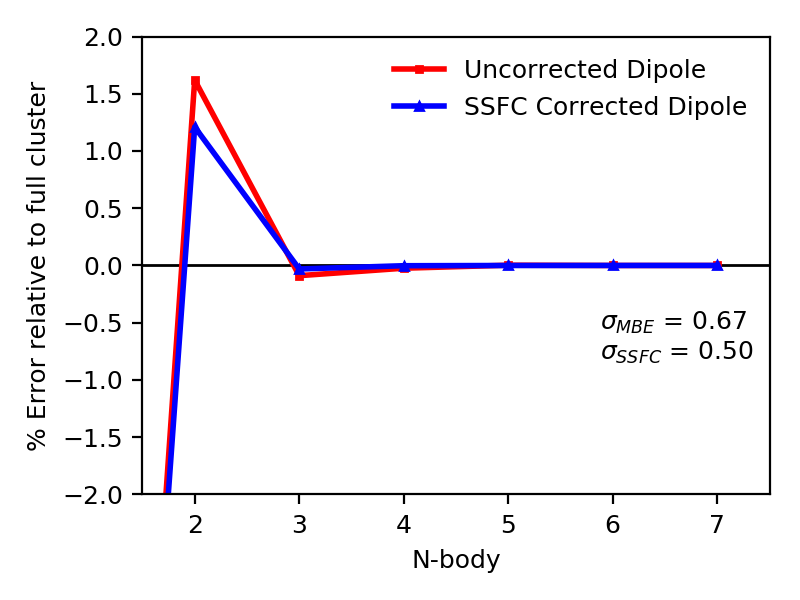
\includegraphics[scale=0.75]{p1/graphs/si/metthi_6_cam_dip.png}
        \caption{MBE and SSFC of dipole moment for (\textit{S})-methylthiirane in a six-water solvent shell. Computed with CAM-B3LYP/aDZ.}
        \label{metthi_6_cam_dip}
    \end{figure}

    \begin{figure}
        \centering
        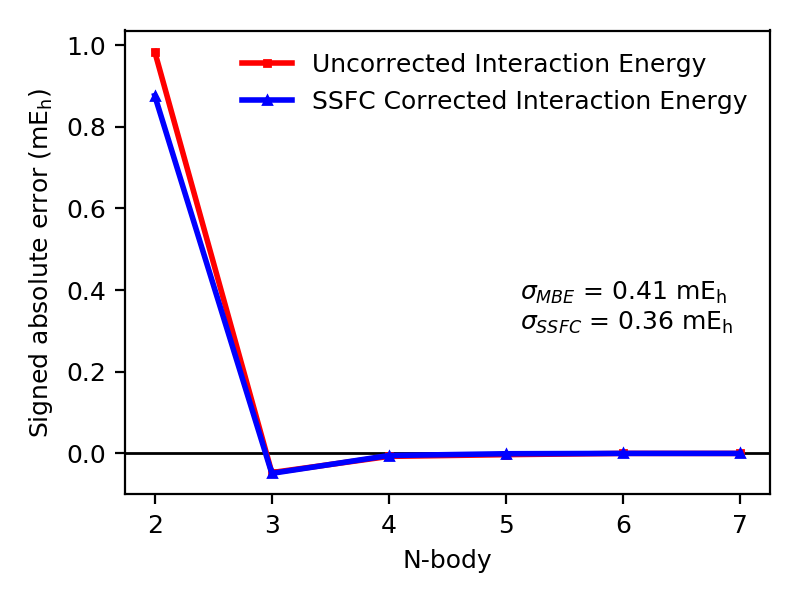
\includegraphics[scale=0.75]{p1/graphs/si/metthi2_6_int.png}
        \caption{MBE and SSFC of interaction energy for snapshot
          \#2 of (\textit{S})-methylthiirane in a six-water solvent shell. Computed with CAM-B3LYP/aDZ.}
        \label{metthi2_6_int}
    \end{figure}
    \begin{figure}
        \centering
        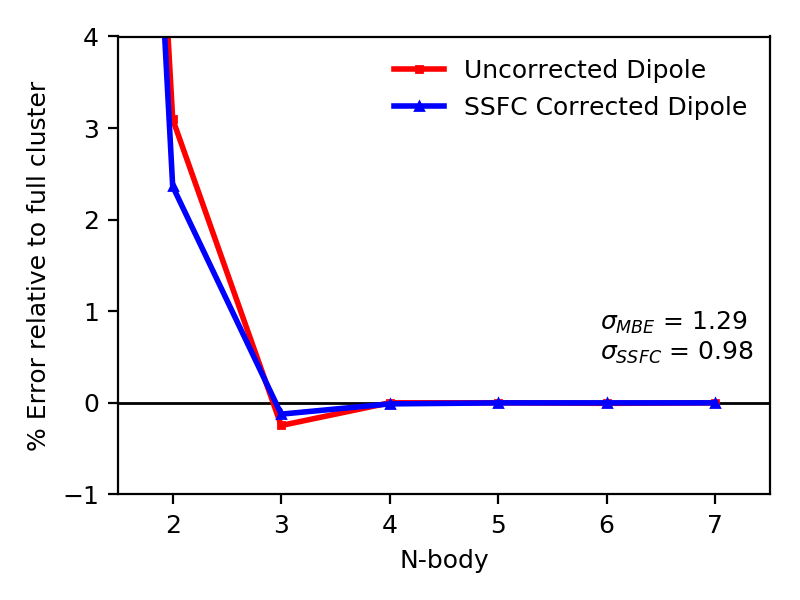
\includegraphics[scale=0.75]{p1/graphs/si/metthi2_6_dip.png}
        \caption{MBE and SSFC of dipole moment for snapshot \#2 of (\textit{S})-methylthiirane in a six-water solvent shell. Computed with CAM-B3LYP/aDZ.}
        \label{metthi2_6_dip}
      \end{figure}

        \begin{figure}
            \centering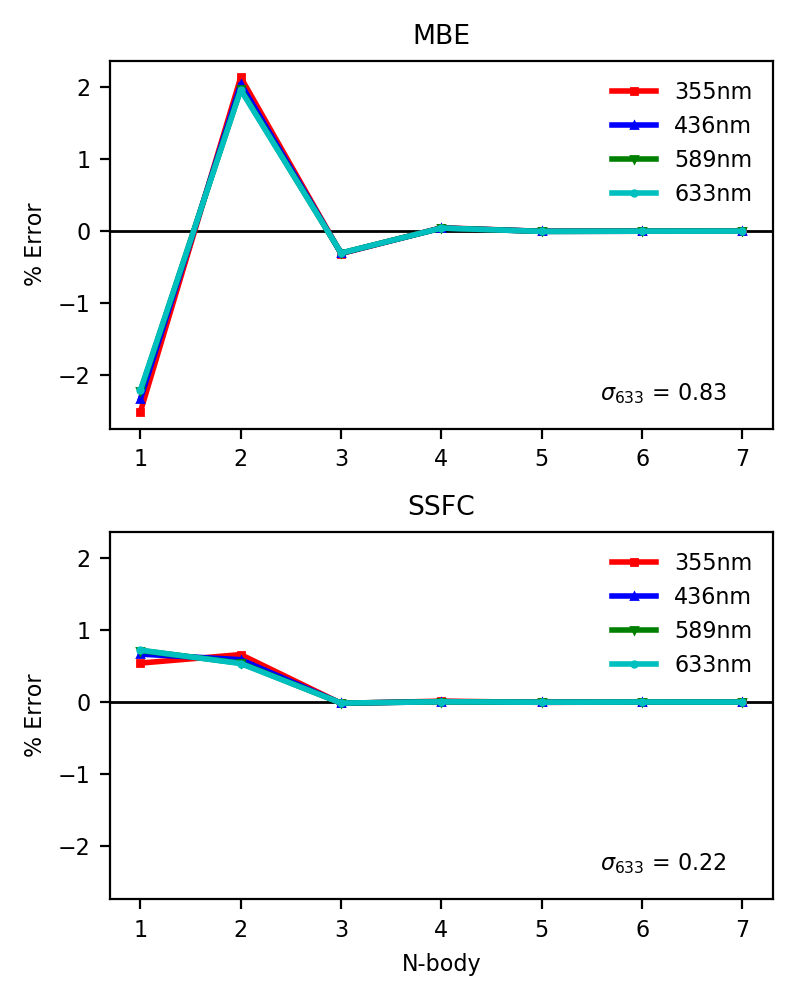
\includegraphics[scale=0.75]{p1/graphs/metthi2_6_pol.png}
            \caption{MBE and SSFC of dynamic polarizabilities for
              snapshot \#2 of (\textit{S})-methylthiirane in a six-water solvent shell. Computed with CAM-B3LYP/aDZ.}
                \label{metthi2_pol}
        \end{figure}

\clearpage
    \subsection{Dimethylallene}
    \begin{figure}
        \centering
        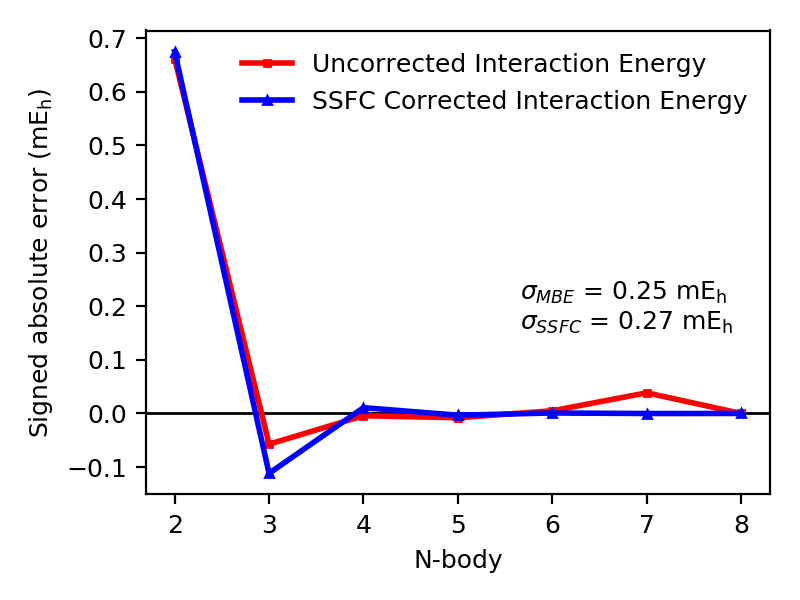
\includegraphics[scale=0.75]{p1/graphs/si/dma_7_b3_int.png}
        \caption{MBE and SSFC of interaction energy for (\textit{M})-dimethylallene in a seven-water solvent shell. Computed with B3LYP/aDZ.}
        \label{dma_7_b3_int}
    \end{figure}
    \begin{figure}
        \centering
        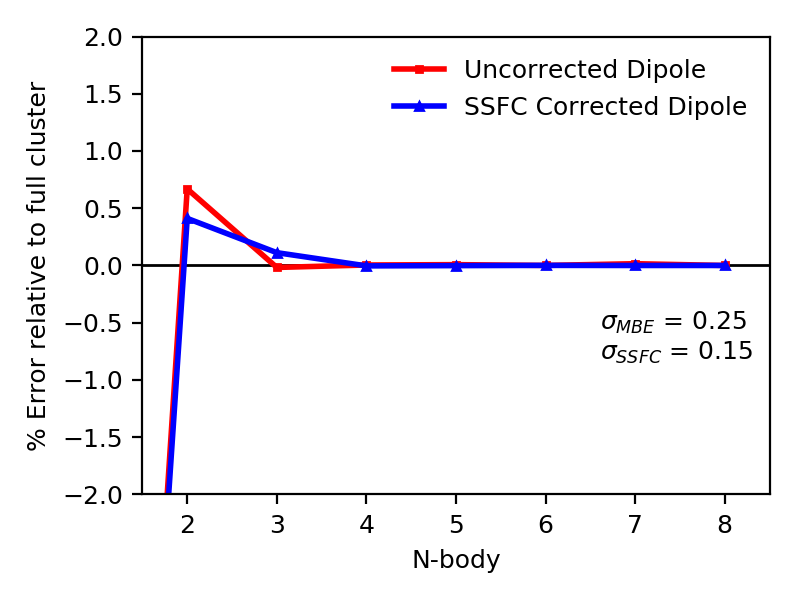
\includegraphics[scale=0.75]{p1/graphs/si/dma_7_b3_dip.png}
        \caption{MBE and SSFC of dipole moment for (\textit{M})-dimethylallene in a seven-water solvent shell. Computed with B3LYP/aDZ.}
        \label{dma_7_b3_dip}
    \end{figure}

    \begin{figure}
        \centering
        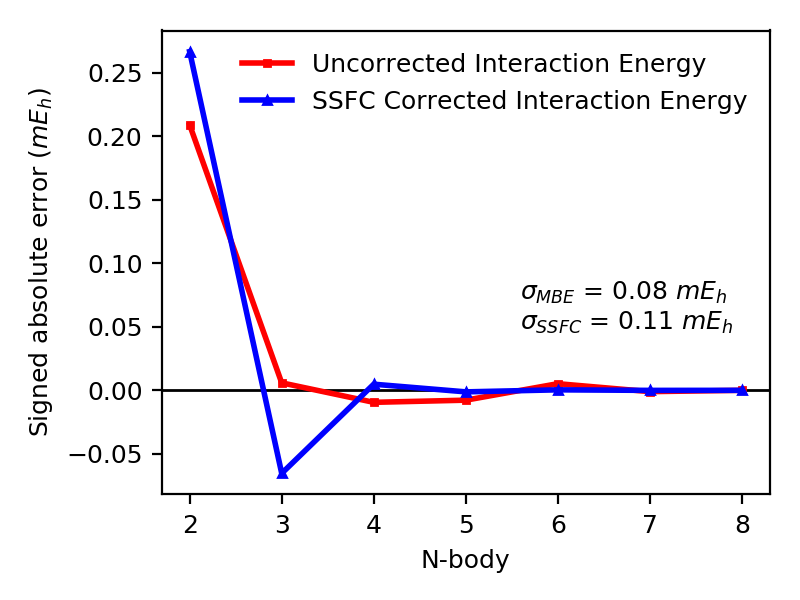
\includegraphics[scale=0.75]{p1/graphs/si/dma_7_cam_int.png}
        \caption{MBE and SSFC of interaction energy for (\textit{M})-dimethylallene in a seven-water solvent shell. Computed with CAM-B3LYP/aDZ.}
        \label{dma_7_cam_int}
    \end{figure}
    \begin{figure}
        \centering
        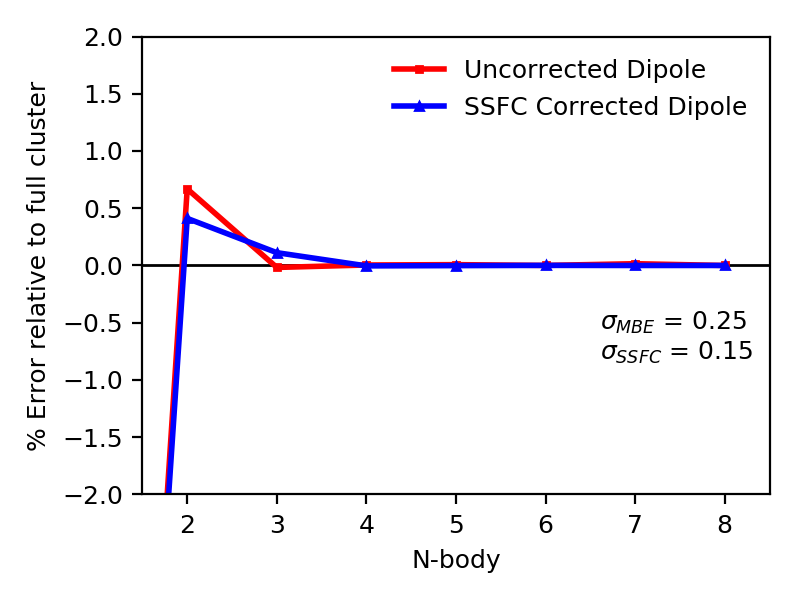
\includegraphics[scale=0.75]{p1/graphs/si/dma_7_cam_dip.png}
        \caption{MBE and SSFC of dipole moment for (\textit{M})-dimethylallene in a seven-water solvent shell. Computed with CAM-B3LYP/aDZ.}
        \label{dma_7_cam_dip}
    \end{figure}

%\newpage
\clearpage
\section{Atomic Coordinates}
\begin{table}[!ht]
%\begin{table}
    \centering
    \caption{Atomic coordinates of (\textit{S})-methyloxirane in a seven-water solvent shell
 (\AA ngstroms)}
    \label{metox_7}
    \begin{tabular}{ c c c c }
    \hline
    \hline
    Atomic & & & \\
    Symbol & X & Y & Z \\
    \hline
	C &  14.600000 &  14.530000 &  15.130000 \\
	O &  14.600000 &  14.530000 &  16.530000 \\
	C &  15.860000 &  14.530000 &  15.850000 \\
	C &  14.520000 &  15.710000 &  14.300000 \\
	H &  13.580000 &  15.710000 &  13.750000 \\
	H &  14.580000 &  16.600000 &  14.920000 \\
	H &  15.350000 &  15.710000 &  13.590000 \\
	H &  14.090000 &  13.640000 &  14.770000 \\
	H &  16.430000 &  13.640000 &  15.590000 \\
	H &  16.430000 &  15.420000 &  15.590000 \\
	O &  11.050000 &  14.880000 &  13.420000 \\
	H &  11.070000 &  14.670000 &  14.350000 \\
	H &  11.780000 &  15.490000 &  13.290000 \\
	O &  18.580000 &  15.280000 &  15.690000 \\
	H &  18.510000 &  14.460000 &  15.220000 \\
	H &  19.390000 &  15.200000 &  16.200000 \\
	O &  17.480000 &  16.470000 &  17.830000 \\
	H &  17.700000 &  15.930000 &  17.070000 \\
	H &  17.110000 &  15.850000 &  18.460000 \\
	O &  11.290000 &  17.480000 &  15.180000 \\
	H &  11.990000 &  16.870000 &  14.960000 \\
	H &  11.360000 &  17.610000 &  16.130000 \\
	O &  16.860000 &  14.160000 &  11.360000 \\
	H &  16.530000 &  13.440000 &  10.810000 \\
	H &  16.400000 &  14.040000 &  12.200000 \\
	O &  12.960000 &  16.070000 &  16.940000 \\
	H &  13.330000 &  15.780000 &  17.770000 \\
	H &  13.710000 &  16.190000 &  16.360000 \\
	O &  16.770000 &  14.240000 &  19.190000 \\
	H &  17.490000 &  13.620000 &  19.050000 \\
	H &  16.010000 &  13.820000 &  18.780000 \\
    \hline
    \hline
    \end{tabular}
\end{table}
\begin{table}
    \centering
    \caption{Atomic coordinates of (\textit{S})-methyloxirane in a seven-water solvent shell (Snapshot \#2)
 (\AA ngstroms)}
    \label{metox2_7}
    \begin{tabular}{ c c c c }
    \hline
    \hline
    Atomic & & & \\
    Symbol & X & Y & Z \\
    \hline
	C &  26.730001 &  26.240002 &  27.180002 \\
	O &  27.889999 &  26.100002 &  26.400002 \\
	C &  26.710003 &  26.310001 &  25.650002 \\
	C &  26.830002 &  27.590000 &  27.900002 \\
	H &  27.570002 &  27.500002 &  28.690002 \\
	H &  27.030001 &  28.430002 &  27.240002 \\
	H &  25.870001 &  27.820000 &  28.340000 \\
	H &  26.700001 &  25.340002 &  27.790001 \\
	H &  26.800001 &  25.380001 &  25.080002 \\
	H &  26.900002 &  27.290001 &  25.220001 \\
	O &  29.530001 &  24.260002 &  27.000000 \\
	H &  29.930000 &  23.990002 &  26.120003 \\
	H &  28.860001 &  24.990002 &  26.860001 \\
	O &  29.590000 &  25.900002 &  24.580002 \\
	H &  28.880003 &  25.980000 &  25.270002 \\
	H &  29.820002 &  24.930000 &  24.450001 \\
	O &  24.010000 &  25.500002 &  25.790003 \\
	H &  23.310001 &  26.220001 &  25.760002 \\
	H &  23.790001 &  24.799999 &  25.120001 \\
	O &  27.560001 &  24.490002 &  30.270002 \\
	H &  26.580002 &  24.660000 &  30.310001 \\
	H &  27.790001 &  24.030001 &  29.410002 \\
	O &  27.170002 &  22.970001 &  25.570002 \\
	H &  27.790001 &  23.140001 &  26.350002 \\
	H &  27.690001 &  23.050001 &  24.720001 \\
	O &  24.600000 &  28.290003 &  23.990002 \\
	H &  24.590000 &  29.290001 &  24.100000 \\
	H &  23.710001 &  27.920000 &  24.260002 \\
	O &  23.850002 &  23.740002 &  27.780001 \\
	H &  24.180002 &  24.550001 &  27.299999 \\
	H &  23.030003 &  23.390003 &  27.320002 \\
    \hline
    \hline
    \end{tabular}
\end{table}
\newpage
\renewcommand*{\arraystretch}{.6}
\begin{table}
    \centering
    \caption{Atomic coordinates of (\textit{S})-methyloxirane in a 7-water solvent shell and two manually reduced H-bonds
 (\AA ngstroms)}
    \label{metox_7_short2}
    \begin{tabular}{ c c c c }
    \hline
    \hline
    Atomic & & & \\
    Symbol & X & Y & Z \\
    \hline
	C &  14.600000 &  14.530000 &  15.130000 \\
	O &  14.600000 &  14.530000 &  16.530000 \\
	C &  15.860000 &  14.530000 &  15.850000 \\
	C &  14.520000 &  15.710000 &  14.300000 \\
	H &  13.580000 &  15.710000 &  13.750000 \\
	H &  14.580000 &  16.600000 &  14.920000 \\
	H &  15.350000 &  15.710000 &  13.590000 \\
	H &  14.090000 &  13.640000 &  14.770000 \\
	H &  16.430000 &  13.640000 &  15.590000 \\
	H &  16.430000 &  15.420000 &  15.590000 \\
	O &  11.050000 &  14.880000 &  13.420000 \\
	H &  11.070000 &  14.670000 &  14.350000 \\
	H &  11.780000 &  15.490000 &  13.290000 \\
	O &  18.601491 &  15.356686 &  16.138508 \\
	H &  18.531491 &  14.536686 &  15.668508 \\
	H &  19.411491 &  15.276686 &  16.648508 \\
	O &  17.480000 &  16.470000 &  17.830000 \\
	H &  17.700000 &  15.930000 &  17.070000 \\
	H &  17.110000 &  15.850000 &  18.460000 \\
	O &  11.805218 &  17.248086 &  15.788585 \\
	H &  12.505218 &  16.638086 &  15.568585 \\
	H &  11.875218 &  17.378086 &  16.738585 \\
	O &  16.860000 &  14.160000 &  11.360000 \\
	H &  16.530000 &  13.440000 &  10.810000 \\
	H &  16.400000 &  14.040000 &  12.200000 \\
	O &  12.960000 &  16.070000 &  16.940000 \\
	H &  13.330000 &  15.780000 &  17.770000 \\
	H &  13.710000 &  16.190000 &  16.360000 \\
	O &  16.770000 &  14.240000 &  19.190000 \\
	H &  17.490000 &  13.620000 &  19.050000 \\
	H &  16.010000 &  13.820000 &  18.780000 \\
    \hline
    \hline
    \end{tabular}
\end{table}
\clearpage
\renewcommand*{\arraystretch}{.5}
\begin{longtable}{ c c c c }
    \caption{Atomic coordinates of (\textit{S})-methyloxirane in a 13-water solvent shell (\AA ngstroms)} \\
    \hline 
    \hline 
    Atomic & & & \\
    Symbol & X & Y & Z \\
    \hline
	C &  14.600000 &  14.530000 &  15.130000 \\
	O &  14.600000 &  14.530000 &  16.530000 \\
	C &  15.860000 &  14.530000 &  15.850000 \\
	C &  14.520000 &  15.710000 &  14.300000 \\
	H &  13.580000 &  15.710000 &  13.750000 \\
	H &  14.580000 &  16.600000 &  14.920000 \\
	H &  15.350000 &  15.710000 &  13.590000 \\
	H &  14.090000 &  13.640000 &  14.770000 \\
	H &  16.430000 &  13.640000 &  15.590000 \\
	H &  16.430000 &  15.420000 &  15.590000 \\
	O &  15.600000 &  19.160000 &  17.660000 \\
	H &  16.160000 &  19.800000 &  17.220000 \\
	H &  15.980000 &  19.070000 &  18.540000 \\
	O &  11.050000 &  14.880000 &  13.420000 \\
	H &  11.070000 &  14.670000 &  14.350000 \\
	H &  11.780000 &  15.490000 &  13.290000 \\
	O &  19.150000 &  17.890000 &  13.810000 \\
	H &  18.590000 &  17.110000 &  13.850000 \\
	H &  19.280000 &  18.130000 &  14.730000 \\
	O &  10.790000 &  14.420000 &  16.000000 \\
	H &  10.100000 &  15.050000 &  16.210000 \\
	H &  11.430000 &  14.510000 &  16.710000 \\
	O &  14.750000 &  19.290000 &  13.750000 \\
	H &  14.910000 &  18.510000 &  14.270000 \\
	H &  15.410000 &  19.920000 &  14.040000 \\
	O &  18.580000 &  15.280000 &  15.690000 \\
	H &  18.510000 &  14.460000 &  15.220000 \\
	H &  19.390000 &  15.200000 &  16.200000 \\
	O &  13.370000 &  14.030000 &  19.010000 \\
	H &  13.860000 &  13.220000 &  18.870000 \\
	H &  12.470000 &  13.750000 &  19.180000 \\
	O &  17.480000 &  16.470000 &  17.830000 \\
	H &  17.700000 &  15.930000 &  17.070000 \\
	H &  17.110000 &  15.850000 &  18.460000 \\
	O &  11.290000 &  17.480000 &  15.180000 \\
	H &  11.990000 &  16.870000 &  14.960000 \\
	H &  11.360000 &  17.610000 &  16.130000 \\
	O &  16.860000 &  14.160000 &  11.360000 \\
	H &  16.530000 &  13.440000 &  10.810000 \\
	H &  16.400000 &  14.040000 &  12.200000 \\
	O &  15.050000 &  12.180000 &  18.300000 \\
	H &  15.510000 &  11.370000 &  18.530000 \\
	H &  15.000000 &  12.160000 &  17.340000 \\
	O &  12.960000 &  16.070000 &  16.940000 \\
	H &  13.330000 &  15.780000 &  17.770000 \\
	H &  13.710000 &  16.190000 &  16.360000 \\
	O &  16.770000 &  14.240000 &  19.190000 \\
	H &  17.490000 &  13.620000 &  19.050000 \\
	H &  16.010000 &  13.820000 &  18.780000 \\
    \hline
    \hline
%    \end{tabular}
\end{longtable}
\renewcommand*{\arraystretch}{1.0}
\begin{table}
    \centering
    \caption{Atomic coordinates of (\textit{S})-methylthiirane in a six-water solvent shell
 (\AA ngstroms)}
    \label{metthi_6}
    \begin{tabular}{ c c c c }
    \hline
    \hline
    Atomic & & & \\
    Symbol & X & Y & Z \\
    \hline
	C &  14.840000 &  14.890000 &  15.500000 \\
	S &  13.220000 &  14.190000 &  14.950000 \\
	C &  13.960000 &  15.880000 &  14.850000 \\
	C &  16.110000 &  14.410000 &  14.820000 \\
	H &  16.400000 &  13.420000 &  15.190000 \\
	H &  15.960000 &  14.340000 &  13.740000 \\
	H &  16.930000 &  15.110000 &  15.020000 \\
	H &  14.910000 &  14.960000 &  16.590000 \\
	H &  13.470000 &  16.630000 &  15.460000 \\
	H &  14.210000 &  16.200000 &  13.840000 \\
	O &  11.050000 &  14.880000 &  13.420000 \\
	H &  11.070000 &  14.670000 &  14.350000 \\
	H &  11.780000 &  15.490000 &  13.290000 \\
	O &  18.580000 &  15.280000 &  15.690000 \\
	H &  18.510000 &  14.460000 &  15.220000 \\
	H &  19.390000 &  15.200000 &  16.200000 \\
	O &  17.480000 &  16.470000 &  17.830000 \\
	H &  17.700000 &  15.930000 &  17.070000 \\
	H &  17.110000 &  15.850000 &  18.460000 \\
	O &  11.290000 &  17.480000 &  15.180000 \\
	H &  11.990000 &  16.870000 &  14.960000 \\
	H &  11.360000 &  17.610000 &  16.130000 \\
	O &  16.860000 &  14.160000 &  11.360000 \\
	H &  16.530000 &  13.440000 &  10.810000 \\
	H &  16.400000 &  14.040000 &  12.200000 \\
	O &  16.770000 &  14.240000 &  19.190000 \\
	H &  17.490000 &  13.620000 &  19.050000 \\
	H &  16.010000 &  13.820000 &  18.780000 \\
    \hline
    \hline
    \end{tabular}
\end{table}
\renewcommand*{\arraystretch}{1.0}
\begin{table}
    \centering
    \caption{Atomic coordinates of (\textit{S})-methylthiirane in a six-water solvent shell (Snapshot \#2)
 (\AA ngstroms)}
    \label{metthi2_6}
    \begin{tabular}{ c c c c }
    \hline
    \hline
    Atomic & & & \\
    Symbol & X & Y & Z \\
    \hline
	C &  26.350002 &  26.090002 &  -26.730001 \\
	S &  28.010002 &  26.670000 &  -26.280001 \\
	C &  26.410000 &  27.530001 &  -26.220001 \\
	C &  25.530003 &  25.180000 &  -25.830002 \\
	H &  24.570000 &  25.030001 &  -26.330002 \\
	H &  26.040001 &  24.220001 &  -25.820000 \\
	H &  25.470001 &  25.540001 &  -24.799999 \\
	H &  26.360001 &  25.760002 &  -27.770002 \\
	H &  26.350002 &  28.360003 &  -26.920002 \\
	H &  25.990002 &  27.750000 &  -25.240002 \\
	O &  25.600002 &  27.190001 &  -29.500000 \\
	H &  24.640003 &  26.960001 &  -29.380001 \\
	H &  26.160002 &  26.620003 &  -28.890001 \\
	O &  23.630001 &  27.710001 &  -24.590000 \\
	H &  22.740002 &  27.680000 &  -25.030001 \\
	H &  24.300001 &  28.140001 &  -25.200003 \\
	O &  24.650002 &  26.170002 &  -22.590000 \\
	H &  24.300001 &  26.840000 &  -23.250000 \\
	H &  25.450001 &  26.550003 &  -22.130001 \\
	O &  24.870003 &  23.340000 &  -28.710001 \\
	H &  24.490002 &  23.500002 &  -29.620001 \\
	H &  25.840000 &  23.600002 &  -28.710001 \\
	O &  28.270000 &  23.770000 &  -28.900002 \\
	H &  28.500002 &  23.220001 &  -28.100002 \\
	H &  28.570002 &  24.710003 &  -28.760002 \\
	O &  29.250002 &  24.520000 &  -24.370001 \\
	H &  30.040001 &  24.410002 &  -24.970001 \\
	H &  28.660002 &  23.710001 &  -24.450001 \\
    \hline
    \hline
    \end{tabular}
\end{table}
\renewcommand*{\arraystretch}{1.0}
\begin{table}
    \centering
    \caption{Atomic coordinates of (\textit{M})-dimethylallene in a seven-water solvent shell
 (\AA ngstroms)}
    \label{dma_7}
    \begin{tabular}{ c c c c }
    \hline
    \hline
    Atomic & & & \\
    Symbol & X & Y & Z \\
    \hline
	C &  12.620000 &  11.350000 &  11.820000 \\
	H &  12.140000 &  10.750000 &  12.590000 \\
	H &  12.940000 &  10.700000 &  11.010000 \\
	H &  11.960000 &  12.140000 &  11.460000 \\
	C &  13.830000 &  12.070000 &  12.410000 \\
	H &  14.840000 &  11.920000 &  12.030000 \\
	C &  13.560000 &  12.880000 &  13.400000 \\
	C &  13.310000 &  13.690000 &  14.390000 \\
	H &  13.320000 &  13.360000 &  15.430000 \\
	C &  13.000000 &  15.130000 &  14.000000 \\
	H &  13.040000 &  15.230000 &  12.920000 \\
	H &  13.730000 &  15.800000 &  14.460000 \\
	H &  12.000000 &  15.320000 &  14.380000 \\
	O &  11.270000 &  13.410000 &  16.900000 \\
	H &  11.740000 &  13.410000 &  17.780000 \\
	H &  10.790000 &  12.540000 &  16.790000 \\
	O &  14.660000 &  14.170000 &   9.530000 \\
	H &  14.070000 &  14.230000 &  10.330000 \\
	H &  14.510000 &  13.290000 &   9.070000 \\
	O &  10.640000 &  13.470000 &  13.400000 \\
	H &   9.840000 &  13.240000 &  13.950000 \\
	H &  11.470000 &  13.210000 &  13.890000 \\
	O &  16.380000 &  10.990000 &  10.790000 \\
	H &  16.430000 &  11.800000 &  11.380000 \\
	H &  15.520000 &  11.010000 &  10.280000 \\
	O &  12.520000 &  17.310000 &  11.280000 \\
	H &  13.360000 &  17.360000 &  10.740000 \\
	H &  12.290000 &  16.350000 &  11.460000 \\
	O &  14.500000 &  12.200000 &  16.330000 \\
	H &  14.410000 &  12.100000 &  17.320000 \\
	H &  15.460000 &  12.130000 &  16.070000 \\
	O &  17.050000 &  14.870000 &  11.040000 \\
	H &  16.120000 &  14.620000 &  10.770000 \\
	H &  17.310000 &  14.370000 &  11.860000 \\
    \hline
    \hline
    \end{tabular}
\end{table}
